\chapter{Results}
\label{chap:results}

\lettrine[lines=4, findent=3pt, nindent=0pt]{I}{n} this chapter results and performance will be discussed. Starting with some metrics about the trained \gls{ml} model, with a particular focus on grouped and ungrouped features, it will then be presented the behavior of the implemented \gls{ids} on real life attacks, taking into consideration what was pointed out in section \ref{subsec:delimitation} about the delimitation of the project. Anyway, the theoretical results achieved remain valid and for this reason form the focus of the chapter.

\section{ML Model Evaluation}
\label{sec:ml-model-evaluation}

The classifier of choice, as discussed in \ref{subsec:classification}, was \textit{Random Forest}. It is particularly interesting to observe the results of the training with ungrouped labels versus the one with grouped labels: the differences in terms of precision and F1 score are remarkable.

\begin{figure}[h!]
   \centering
   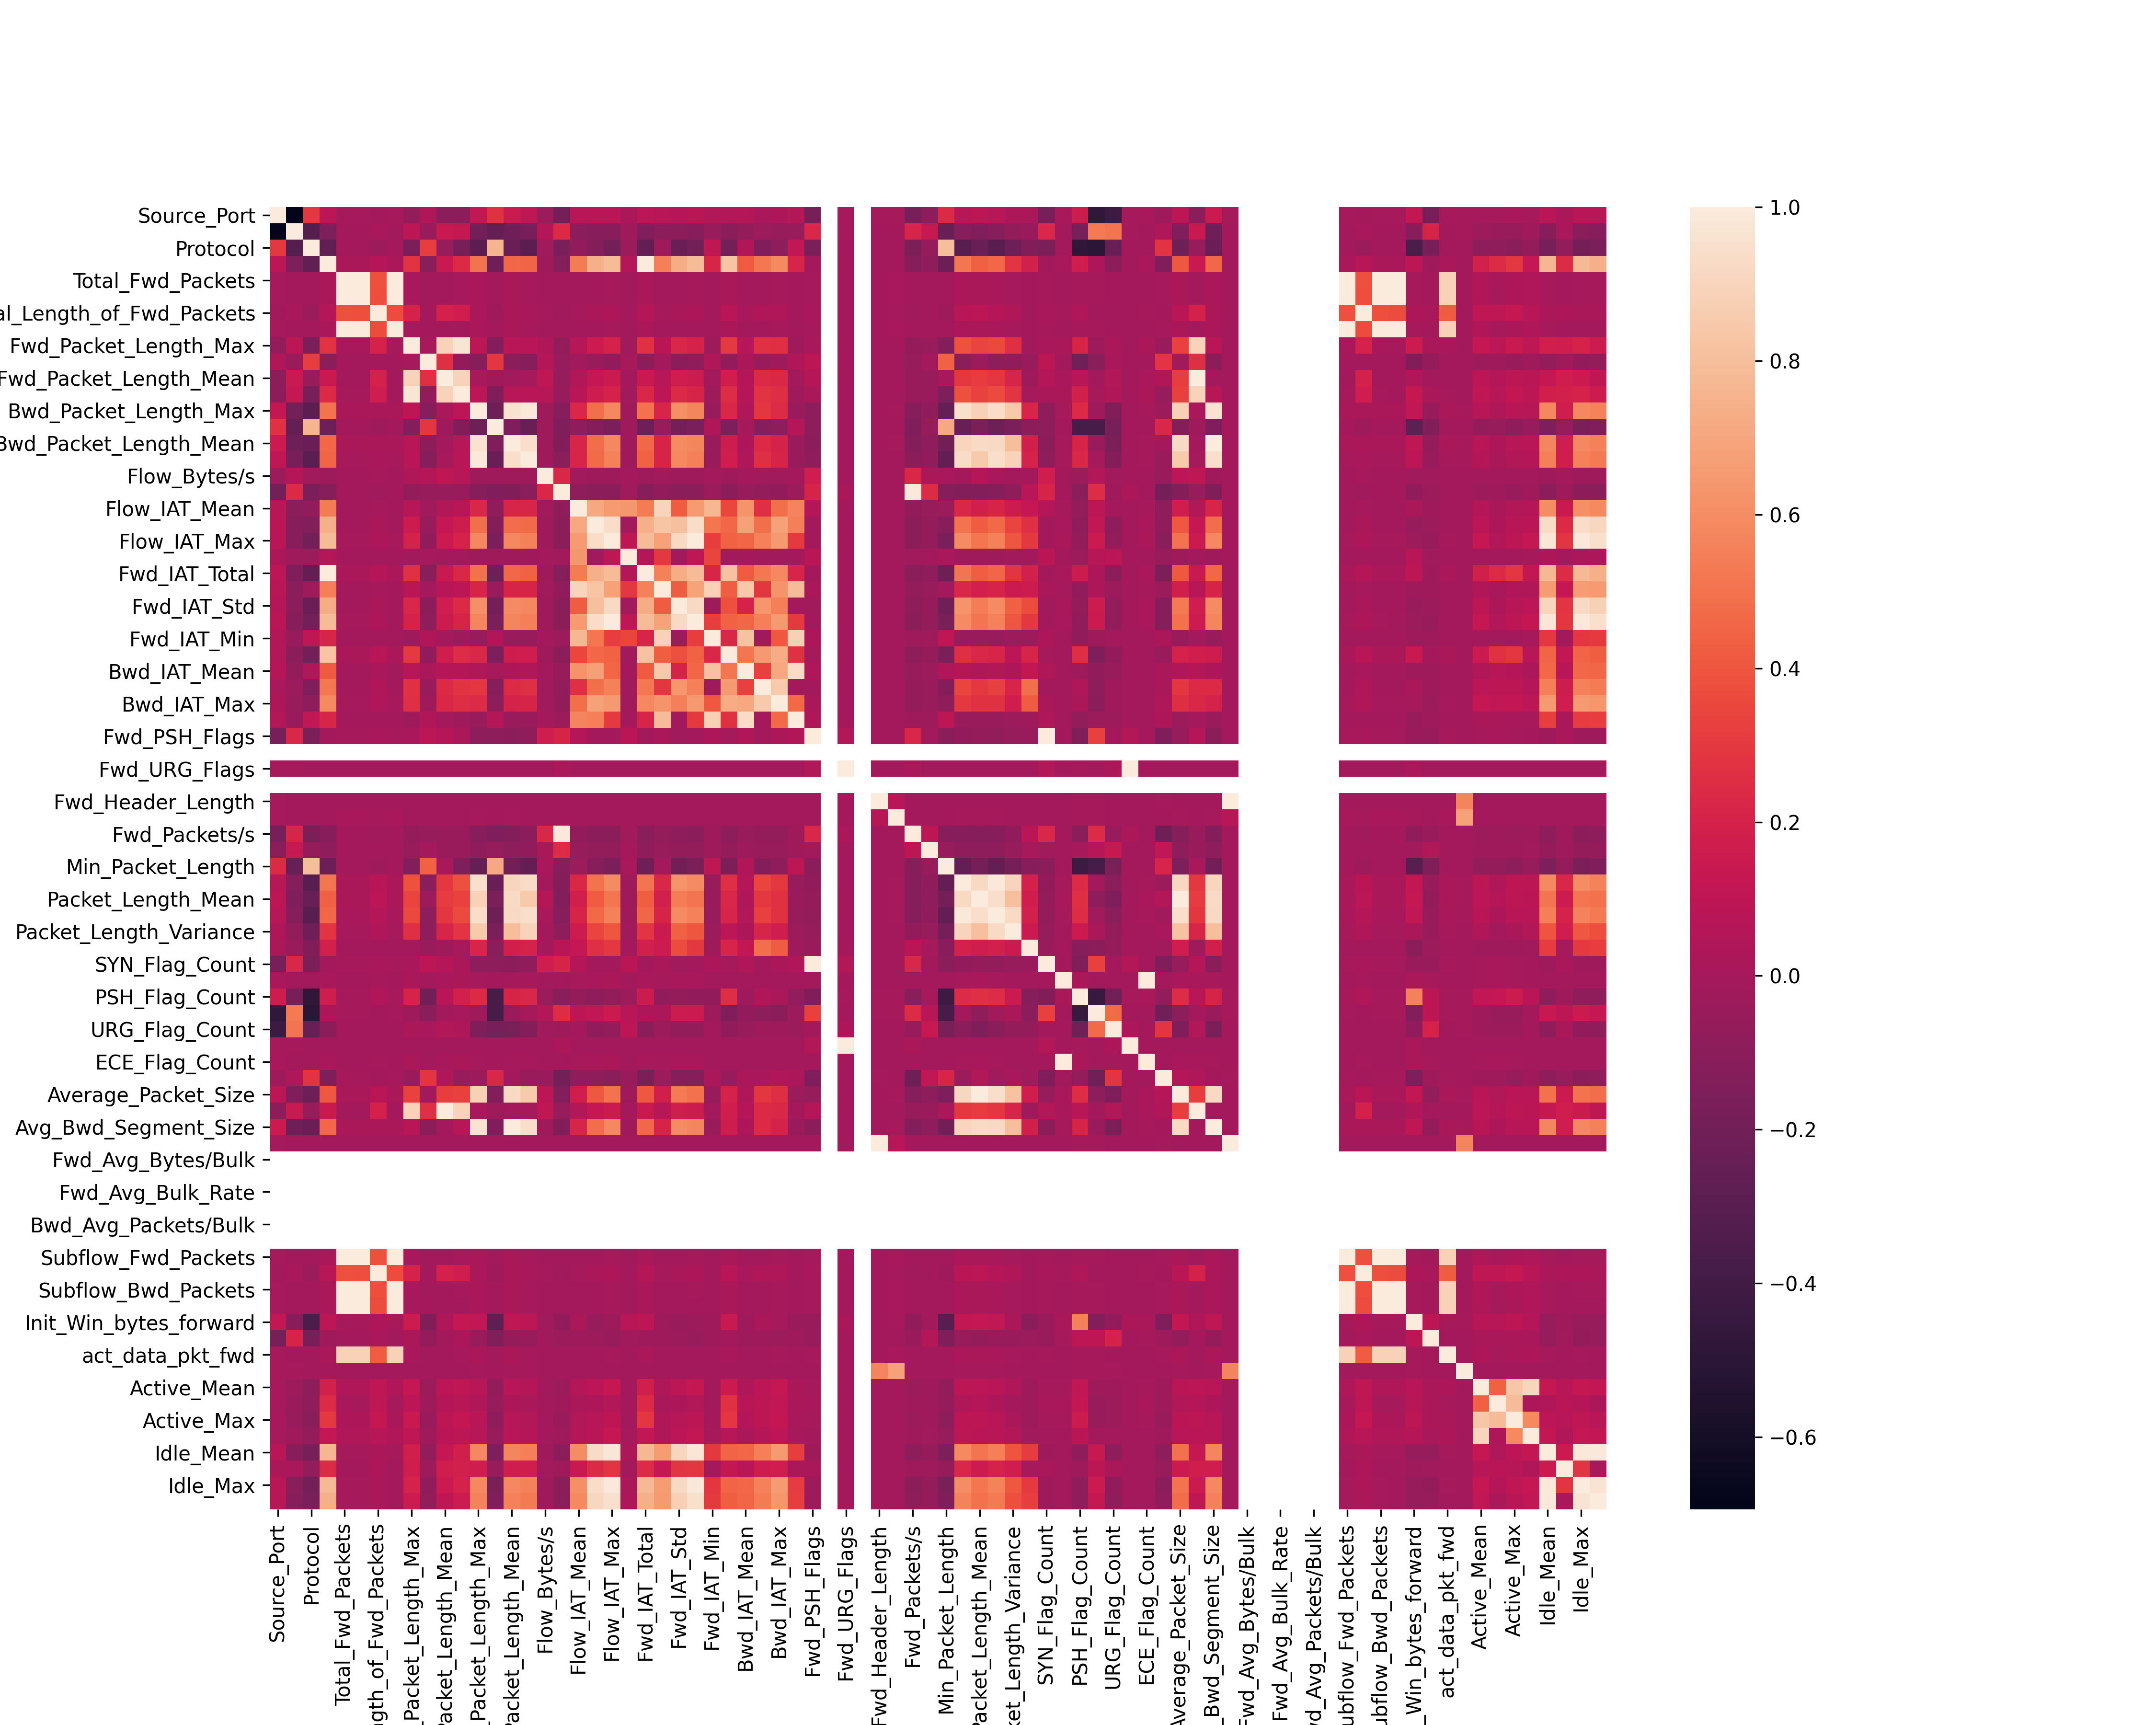
\includegraphics[scale=0.5]{assets/figures/chapter3/heatmap-all.png}
   \caption{CICIDS2017 Feature Correlation Matrix (heatmap)}
   \label{fig:feature-heatmap}
\end{figure}

\subsection{Ungrouped Labels Model}
\label{subsec:ungrouped-training}

\begin{figure}[h!]
   \centering
   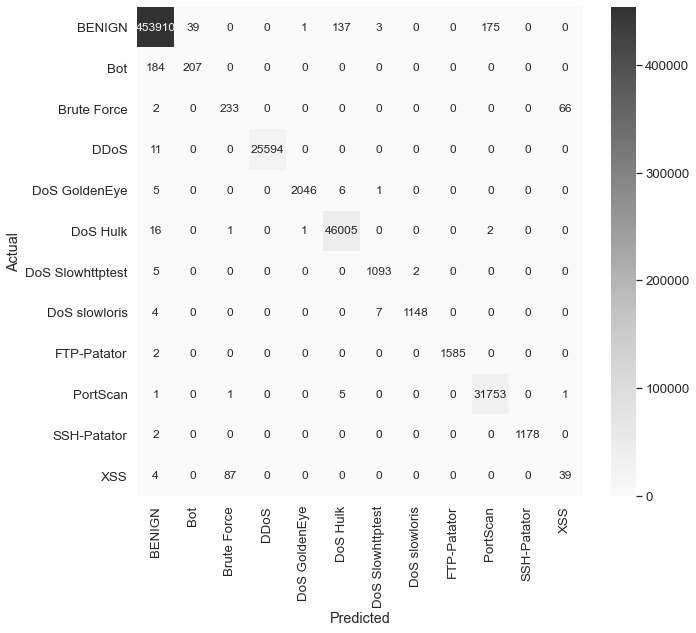
\includegraphics[scale=0.62]{assets/figures/chapter3/ungrouped_confusion_matrix.png}
   \caption{Confusion Matrix of the Random Forest model trained using CICIDS2017 dataset with ungrouped features}
   \label{fig:ungrouped-confusion-matrix}
\end{figure}

\begin{table}[h!]
   \centering
   \begin{tabular}{l|llll}
       \toprule 
       Traffic Label & Precision (\%) & Recall (\%) & F1 Score (\%) \\
       \midrule
       \rowcolor{black!10} \texttt{Benign} & 99.9507 & 99.9199 & 99.9353 \\
       \texttt{Bot} & 82.4219 & 53.9642 & 65.2241 \\
       \rowcolor{black!10} \texttt{Brute Force} & 100.0000 & 99.9277 & 99.9638 \\
       \texttt{DDoS} & 100.0000 & 99.9727 & 99.9863 \\
       \rowcolor{black!10} \texttt{DoS GoldenEye} & 99.7047 & 99.9404 & 99.8224 \\
       \texttt{DoS Hulk} & 99.4456 & 99.9717 & 99.7080 \\
       \rowcolor{black!10} \texttt{DoS Slowloris} & 99.2991 & 98.6079 & 98.9523 \\
       \texttt{FTP-Patator} & 100.0000 & 99.9727 & 99.9863 \\
       \rowcolor{black!10} \texttt{Port Scan} & 99.7047 & 99.9404 & 99.8224 \\
       \texttt{SSH-Patator} & 99.4456 & 99.9717 & 99.7080 \\
       \rowcolor{black!10} \texttt{XSS} & 99.2991 & 98.6079 & 98.9523 \\
       \bottomrule
   \end{tabular}
   \caption{\textit{Random Forest} trained model metrics on CICIDS2017 (ungrouped) features}
   \label{tab:ungrouped-metrics}
\end{table}

\subsection{Grouped Labels Model}
\label{subsec:grouped-training}

\begin{figure}[h!]
   \centering
   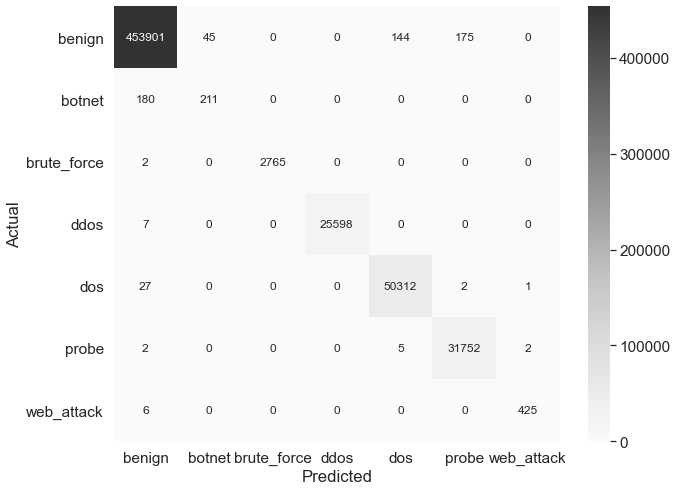
\includegraphics[scale=0.52]{assets/figures/chapter3/grouped_confusion_matrix.png}
   \caption{Confusion Matrix of the Random Forest model trained using CICIDS2017 dataset with grouped features}
   \label{fig:grouped-confusion-matrix}
\end{figure}

asdasd
\begin{table}[h!]
   \centering
   \begin{tabular}{l|llll}
       \toprule 
       Traffic Label & Precision (\%) & Recall (\%) & F1 Score (\%) \\
       \midrule
       \rowcolor{black!10} \texttt{Benign} & 99.9507 & 99.9199 & 99.9353 \\
       \texttt{Botnet} & 82.4219 & 53.9642 & 65.2241 \\
       \rowcolor{black!10} \texttt{Brute Force} & 100.0000 & 99.9277 & 99.9638 \\
       \texttt{DDoS} & 100.0000 & 99.9727 & 99.9863 \\
       \rowcolor{black!10} \texttt{DoS} & 99.7047 & 99.9404 & 99.8224 \\
       \texttt{Probe} & 99.4456 & 99.9717 & 99.7080 \\
       \rowcolor{black!10} \texttt{Web Attack} & 99.2991 & 98.6079 & 98.9523 \\
       \bottomrule
   \end{tabular}
   \caption{\textit{Random Forest} trained model metrics on CICIDS2017 (grouped) features}
   \label{tab:grouped-metrics}
\end{table}

 \noindent This table layout allows visualization of the algorithm's performance. Each row of the matrix represents the instances in an \textit{actual} class, while each column represents the instances in a \textit{predicted} class. As the name suggests, the graph makes easier to see whether the model is confusing two classes: in this case the precision is remarkable, upholding the choice made.


 \section{Feature Weight}
\label{sec:feature-weight}

\textcolor{dimgray}{\lipsum[1-2]}